\documentclass[myclassdoc,debug]{rjparticle}
%use the following command when typesetting your paper:
%\documentclass{rjparticle}
\usepackage{graphicx}

\title{Wobbling Nucleus II} 

\author[1,2,$a$]{R. Poenaru}
\author[2,3,$b$]{A. A. Raduta}

\affil[1]{Doctoral School of Physics, University of Bucharest, Bucharest, Romania\\
\email[a]{robert.poenaru@drd.unibuc.ro} }
\affil[2]{Department of Theoretical Physics - \textit{Horia Hulubei} National Institute for Physics and Nuclear Engineering, M\u{a}gurele-Bucharest, Romania\\
\email[b]{raduta@nipne.ro} (corresponding author)}
\affil[3]{Academy of Romanian Scientists, Bucharest, Romania}

\keywords{Nuclear Structure, Triaxial Nuclei, Wobbling Motion, Parity Symmetry, Signature Partners, Strong Deformation}

\pacs{01.30.-y, 01.30.Ww, 01.30.Xx, 99.00.Bogus}

\hyphenation{rjp-ar-ti-cle}

%%%%%%%%%%%%%%%%%%%%%%%%%%%%%%%%%%%%%%%%%%%%%%%%%%%%%%%%%%%%%%%%%%%%%%%%%%%%%%%
%Please, do not remove the following lines!
%%%%%%%%%%%%%%%%%%%%%%%%%%%%%%%%%%%%%%%%%%%%%%%%%%%%%%%%%%%%%%%%%%%%%%%%%%%%%%%
%\RJPVolume{63}{2018}
%\RJPNumber{1-2}
%\RJPPages{}{}
\columntitle{Wobbling Nucleus II}
%\date{}
%\dedication{}
%\domaintitle{}
%\keywords{}
%\pacs{01.30.-y, 01.30.Ww, 01.30.Xx, 99.00.Bogus}
%%%%%%%%%%%%%%%%%%%%%%%%%%%%%%%%%%%%%%%%%%%%%%%%%%%%%%%%%%%%%%%%%%%%%%%%%%%%%%%

\begin{document}
%%%%%%%%%%%%%%%%%%%%%%%%%%%%%%%%%%%%%%%%%%%%%%%%%%%%%%%%%%%%%%%%%%%%%%%%%%%%%%%
%Please, remove these lines when typesetting your document!
%%%%%%%%%%%%%%%%%%%%%%%%%%%%%%%%%%%%%%%%%%%%%%%%%%%%%%%%%%%%%%%%%%%%%%%%%%%%%%%
\lstset{%
basicstyle=\small,
language=[AlLaTeX]TeX,
columns=fullflexible,
%keepspaces=true,
showspaces=true,
showstringspaces=false,
keywordstyle=[2]\ttfamily,
identifierstyle=,
texcsstyle=*\ttfamily,
commentstyle=\color{gray},
string=[s]<>,
morestring=[b]',
stringstyle=\emph,
breaklines=true,
deletekeywords={list},
moretexcs={authnote,keywords,pacs},
}
%%%%%%%%%%%%%%%%%%%%%%%%%%%%%%%%%%%%%%%%%%%%%%%%%%%%%%%%%%%%%%%%%%%%%%%%%%%%%%%
\maketitle

\begin{abstract}
Abstract 1.
\end{abstract}

\section{Introduction compatibility}
The Romanian Journal of Physics (RJP) style was designed to allow authors, who use mainly \LaTeX ~for typesetting their papers, to  submit contributions to this journal of the Romanian Academy Publishing House. At the same time, by using this style, the authors will have much better control over the final layout of their paper and they will know the number of pages their contribution will occupy when bound in the printed volume (of course only if their contribution will first be accepted and recommended by RJP's referees for publication). \cite{knuth} and \cite{dknuthhp} are citations.

\section{Examples for various Environments}
This section includes examples of different environments containing media and data material (the copyright of which is already owned by RJP) much needed in any good scientific publication. For instance below (in figure \ref{pic1}) we present a \textit{figure} environment as it must appear in every contribution submitted to our journal (this picture is in PNG format so compiling must be done using \textit{pdflatex} command rather than the usual \textit{latex} command or one should specify the \textbf{pdftex} driver when loading the \textbf{graphicx} package).
\begin{figure}[h!tb]
\centering
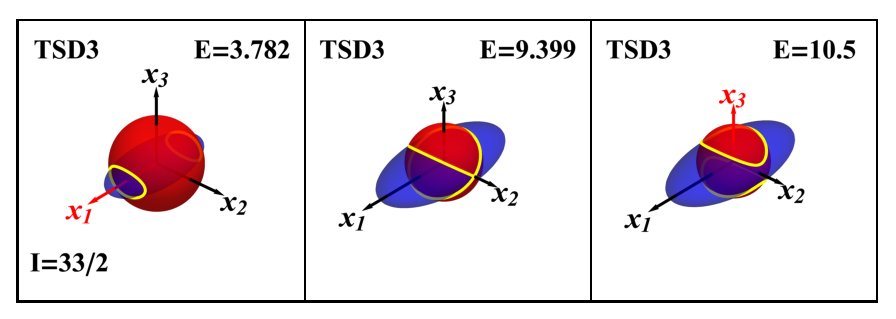
\includegraphics[width=0.8\textwidth]{tsd3_spin1.eps}
\caption{This is a sample picture taken from RJP volume \textbf{50}(1-2) from page 129 (2005).It illustrates (hashed areas) the instability domains for a series of nonlinear Schr\"odinger equations determined using the deterministic approach to modulational instability.}
\label{pic1}
\end{figure}


\begin{table}[h!t]%
\caption{This table is taken from RJP volume \textbf{50}(1-2) from page 43 (2005). It gives the ``
\textit{number of bound states dependence on the radius of space curvature for $\alpha = 0.005$, $U_0 = 1$}''.}
\centering
\begin{tabular}{|c|c|}
\hline
Value $\rho$ & Value $\varepsilon$ \cr
\hline
$\rho = 50$ & -- \cr
$\rho = 100$ & -- \cr
$\rho = 250$ & $\varepsilon_1 = 0.0289$ \cr
$\rho = 400$ & $\varepsilon_1 = 0.3772$ \cr
$\rho = 1000$ & $\varepsilon_1 = 0.4142$, $\varepsilon_2 = 0.8495$ \cr
\hline
\end{tabular}
\label{table1}
\end{table}


\begin{acknowledgement}
The author(s) would like to dedicate this at the Romanian Academy Publishing House.
\end{acknowledgement}


\begin{thebibliography}{99}
\bibitem{knuth}D. E. Knuth, D. R. Bibby, ``\textit{The \TeX book}'', 20th edn. (AMS \& Addison-Wesley Publ. Co., 1991).
\bibitem{dknuthhp} D. E. Knuth homepage: \href{http://www-cs-faculty.stanford.edu/~knuth/}{\small\ttfamily www-cs-faculty.stanford.edu/\~{}knuth}.

\end{thebibliography}


\end{document}